\documentclass[../../main.tex]{subfiles}

\begin{document}

\setchapterpreamble[u]{\margintoc}

\chapter{排序的应用}

在链表中,我们已经实现了某些基础排序的应用,在本章我们通过简单介绍一下排序的应用。实际上排序更多的是
一种思想,我们更应该掌握使用排序的思想解决问题。

\section{基于比较的排序算法}

本节首先基于\href{https://leetcode.cn/problems/sort-an-array/}{排序数组}阐述所有的基于比较的排序算法。

\subsection{插入排序}

插入排序的做法相当简单,我们只需要理解其循环不变量就可以解决该问题,其循环不变量为:\texttt{[0, i)}
是有序的,我们每次将\texttt{nums[i]}插入到\texttt{[0, i)}中,然后\texttt{i++},直到\texttt{i}等于
\texttt{nums.length}。

\lstinputlisting[language=C++]{code/sort-an-array-insertion-sort.cpp}

\subsection{选择排序}

选择排序的做法也相当简单,我们同样需要理解其循环不变量,其循环不变量为:\texttt{[0, i)}是有序的,
我们每次选择\texttt{[i, nums.length)}中的最小值,然后将其与\texttt{nums[i]}交换,然后\texttt{i++},
直到\texttt{i}等于\texttt{nums.length}。

\lstinputlisting[language=C++]{code/sort-an-array-selection-sort.cpp}

\section{快速排序的应用}

\subsection{\href{https://leetcode.cn/problems/kth-largest-element-in-an-array/}
{数组中的第K个最大元素}}

我们应该如何选择数组中的第K个最大元素呢?我们可以先对数组进行排序,然后选择第K个元素,但是这样的
时间复杂度为$O(n\log n)$,我们可以使用快速排序的思想,每次选择一个元素,将数组分为两部分,然后
判断第K个元素在哪一部分,然后递归的进行查找。这样时间的复杂度为$O(n)$\sidenote{要证明这个时间
的复杂度为$O(n)$,需要通过概率来证明,证明方法可以参考算法导论。}。

我们仍然以例子说明,我们取末尾的元素作为\texttt{pivot},然后按照这个数字,对数组进行分割,然后
递归地进行处理。假设我们对最初的数组完成了以下的分割,并得到了这个\texttt{pivot}的位置,如下图
所示:

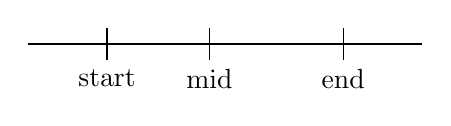
\begin{tikzpicture}
  \draw (0,0) -- (5,0);
  \draw (2.3,-0.2) node[below] {mid} -- (2.3,0.2);
  \draw (1,0.2) -- (1,-0.2) node[below] {start};
  \draw (4,0.2) -- (4,-0.2) node[below] {end};
\end{tikzpicture}


如上图所示,我们首先计算出当前的\texttt{mid}距离\texttt{start}的距离,其值为
\texttt{mid - start + 1},然后我们对这个值进行相应的判断:

\begin{itemize}
  \item 如果其等于\texttt{k},那么证明我们找到了第\texttt{k}个最大元素。
  \item 如果其大于\texttt{k},那么我们递归的对左边的数组进行处理,首先我们要确定新的
  \texttt{start}和\texttt{end},\texttt{start}不变,\texttt{end}变为\texttt{mid - 1}。
  同时\texttt{k}不变。
  \item 如果其小于\texttt{k},那么我们递归的对右边的数组进行处理,首先我们要确定新的
  \texttt{start}和\texttt{end},\texttt{start}变为\texttt{mid + 1},\texttt{end}不变。
  同时\texttt{k}变为\texttt{k - (mid - start + 1)}。
\end{itemize}

然后,我们就可以给出如下的代码:

\lstinputlisting[language=C++]{code/kth-largest-element-in-an-array.cpp}

\end{document}
